%\documentclass[12pt,a4paper]{article}
\documentclass[journal]{IEEEtran}

\title{%
  Arduinoøving 3 \\
  \large IELET1002 - Datateknikk \\
  }
\author{Gunnar Myhre, BIELEKTRO}

\usepackage{graphicx}
\usepackage[utf8]{inputenc}
\usepackage[norsk]{babel}
\usepackage{amsmath}
\usepackage[siunitx]{circuitikz}
\graphicspath{ {./arduino_img} }
\usepackage[style=ieee]{biblatex}

\setlength\parindent{0pt}

%https://github.com/trihedral/ArduinoLatexListing/blob/master/arduinoLanguage.tex
% Patch for æøå: \lstset{texcl=true}
\input{arduinoLanguage.tex}

\begin{document}
  \maketitle
  \section{Introduksjon}
  I arduinoøving 3 har eg laga eit reaksjonsspel for to spelerar. Eg har brukt to trykknappar,
  ein OLED-skjerm, ein piezoelektrisk buzzer og ein RGB-led. Dette dokumentet inneheld ein
  demonstrasjon av funksjonaliteten samt eit refleksjonsnotat om kva eg har lært.
  \section{Demonstrasjon}
  Når arduinoen skruast på startar spelet opp i ein intromeny. Her visast ein tittel, og
  den midterste linja av tekst skiftar mellom to forskjellige strengar, som forklarer brukaren
  kva som er formålet med spelet.
  \begin{figure}[!h]
    \begin{center}
      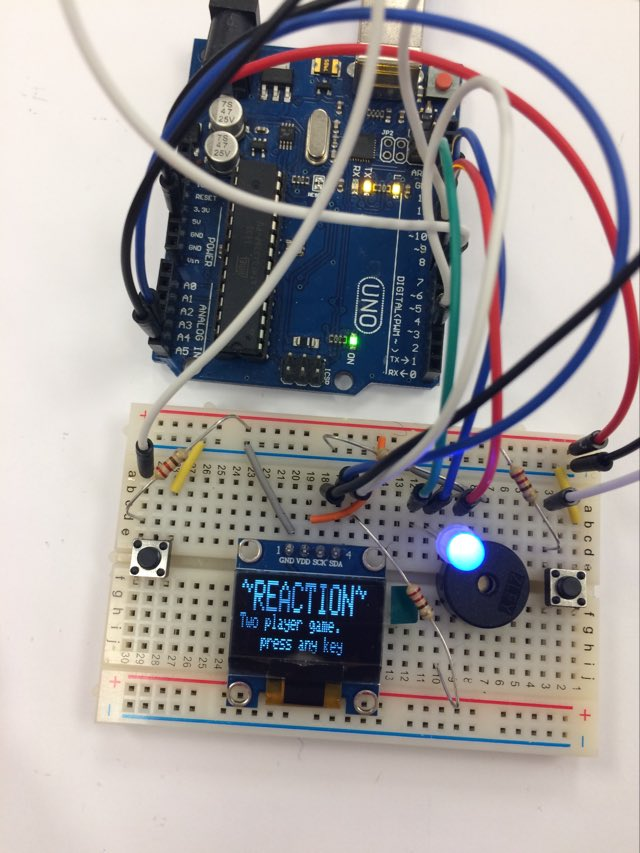
\includegraphics[scale=0.2]{03_menu}
      \caption{Hovedmenyen som dukker opp når du starter.  Når ein av knappane
      vert påtrykt går spelet vidare. LED-en skruast av, og skjermen seier}
    \end{center}
  \end{figure}
  \begin{figure}[!h]
    \begin{center}
      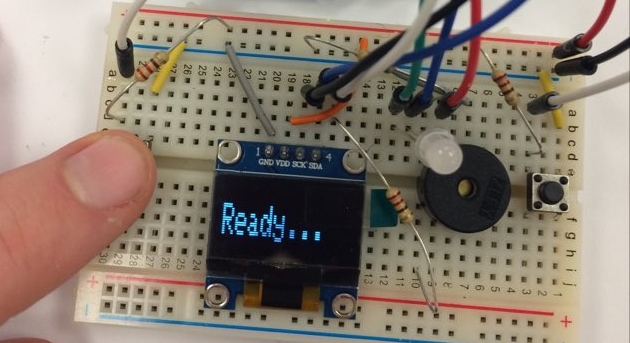
\includegraphics[scale=0.2]{03_ready}
      \caption{Skjermen ber deg gjere deg klar}
    \end{center}
  \end{figure}
  \begin{figure}[!h]
    \begin{center}
      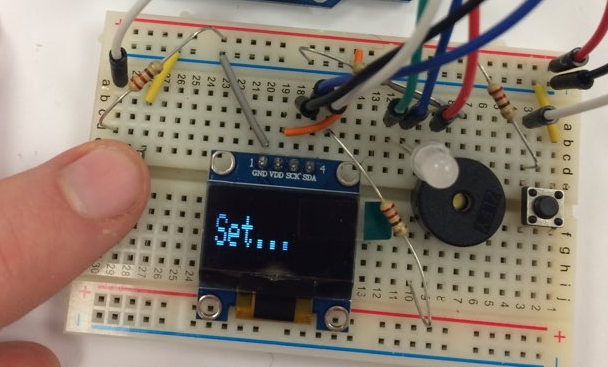
\includegraphics[scale=0.2]{03_set}
      \caption{Like før nå....  Etter $1,5$ sekund starter ein tilfeldig
      periode, skjermen seier \textit{Set...}}
    \end{center}
  \end{figure}
  \begin{figure}[!h]
    \begin{center}
      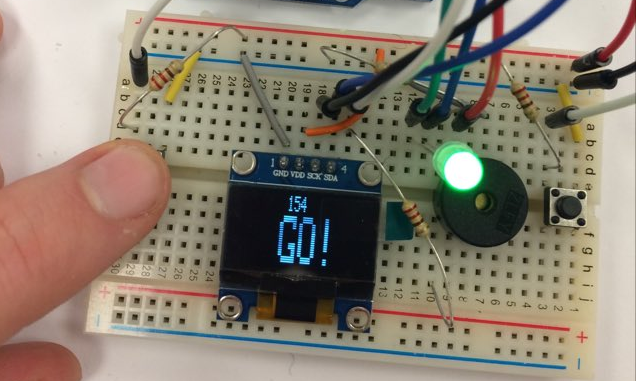
\includegraphics[scale=0.2]{03_go}
      \caption{Skjermen seier til slutt (etter eit tilfeldig tidsintervall som
      er skjult for spelarane) \textbf{GO!}, og då er det opp til førstemann å
      trykke. Eit tal teler ned frå $1000$, og dette er poengsummen du kan
      tjene. Dersom du venter for lenge vert denne poengsummen $0$. LED-en
      lyser grønt for å vise at du skal trykke.}
    \end{center}
  \end{figure}
  \begin{figure}[!h]
    \begin{center}
      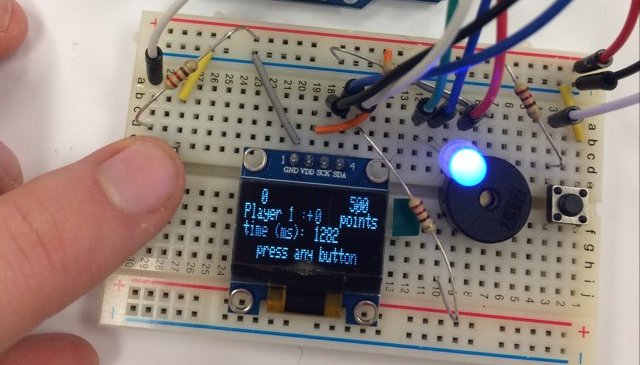
\includegraphics[scale=0.2]{03_announce}
      \caption{ Skjermen viser informasjon om kven som trykte først, kva for
      reaksjonshastigheit og kor mange poeng denne spelaren fekk. Øverst på
      skjermen kan ein også sjå den totale poengsummen til dei to spelarane.}
    \end{center}
  \end{figure}
  \begin{figure}[!h]
    \begin{center}
      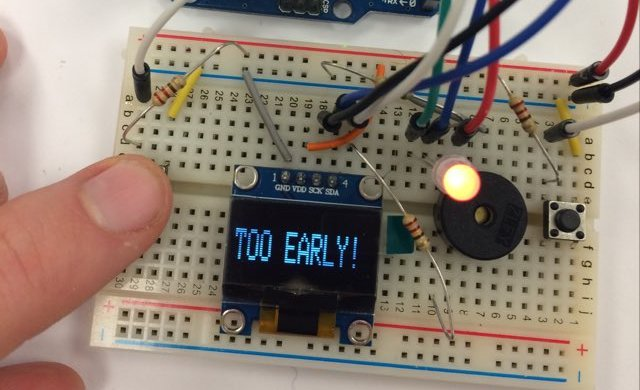
\includegraphics[scale=0.2]{03_fail}
      \caption{Dersom ein spelar trykker før leden lyser grønt blinker LED-en raudt}
    \end{center}
  \end{figure}
  \begin{figure}[!h]
    \begin{center}
      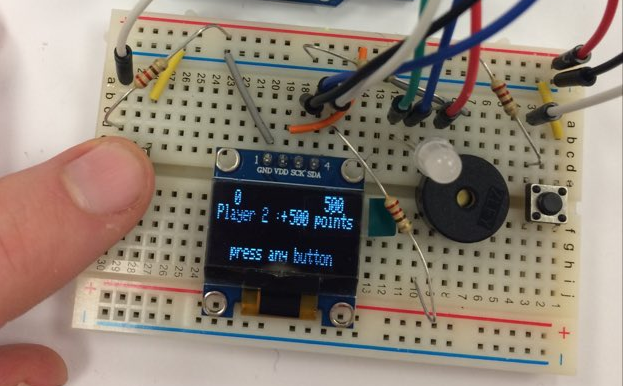
\includegraphics[scale=0.2]{03_penalty}
      \caption{Om du trykker for tidleg får motstandaren 500 poeng}
    \end{center}
  \end{figure}
  \begin{figure}[!h]
    \begin{center}
      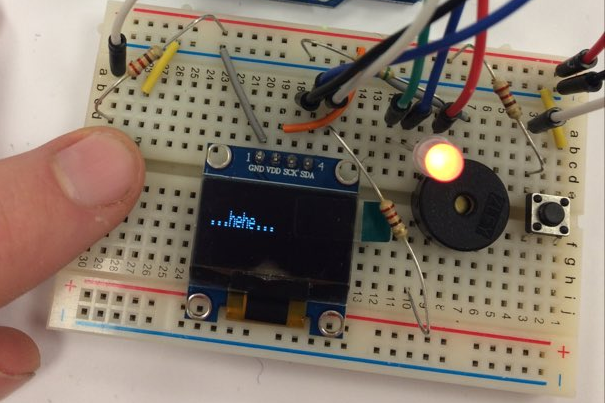
\includegraphics[scale=0.2]{03_trick}
      \caption{$33\%$ av rundene inneholder eit \textit{trick}, då går LED-en til
      raudt når den vanlegvis skulle gått til GO. Om ein spelar trykker på dette
      tidspunktet vil motstandaren få poeng.}
    \end{center}
  \end{figure}

  \subsection{Implementasjon}
  Programmet er implementert etter visse prinsipp:
  \begin{itemize}
    \item Eg ville unngå å bruke delay-funksjonen sidan den stopper opp eksekvering
      av programmet og gjer timing veldig vanskelig når ein har litt meir avanserte
      prosjekter og vil ha friheten til å ha forskjellige frekvensar simultant.
    \item Eg ville til ein viss grad innkapsulere implementasjonsdetaljar for å 
      gjere programmet lettare å endre på eit høgare nivå. Dette gjorde eg
      vha. klasser, \textit{structs} og objektinstansar av desse, og med bruk av \textit{enum} for å
      namngje tilstandsvariablane.
    \item Eg ville dele programmet opp slik at delar av det var plassert på
      logiske plasseringar. For eksempel er all logikken som hører til
      seriellkommunikasjon plassert på ein plass, og derfor enkel å deaktivere
      med ein konstant \textit{PRINT\_TO\_SERIAL}
    \item Eg valgte meg tilstandsmaskiner med eit gitt antal tilstandar som ein
      abstraksjon over maskinvara. Ein fordel med dette er at det er lettare
      å tidsprofilere, debugge og utvide.
  \end{itemize}

  Eg laga også musikk til spelet. Denne er generert og bruker eit triks der eg 
  \textit{bit-shifter} to variablar saman, og dermed får emergent kompleksitet
  over tid. Dette høyrast kult ut når du speler det av i ein høgtalar. Eg triksa
  det til så eg fekk to versjonar av ein sang eg likte, men med forskjellig intensitet,
  og dette brukast i forskjellige delar av spelet for å oppnå dramatisk effekt.



  \subsection{Diskusjon og refleksjon}
  Eg har lært mykje av denne øvinga, sidan den fekk meg til å utforske forskjellige
  programmeringsarkitekturvalg for C++. Eg lærte meg mellom anna
  \begin{itemize}
    \item enum
    \item class
    \item struct
    \item bruk av switch-case, mtp. scope.
  \end{itemize}
  Den beste abstraksjonen eg fann i oppgva var nok å bruke tilstandsmaskiner
  som kvar fekk tildelt éin oppdatering av tilstand i løpet av hovedloopen i
  programmet.  Det gjorde det enkelt å skjønne kor programmet brukte mest tid
  eller eventuelt hang seg opp, og det gjorde det enklare å forstå feil som
  oppsto.  Mykje av dette skyldast at alle variablane i ein gitt tilstand er
  kjent frå augeblikket programmet vert kompilert, og det var derfor ofte lett
  å sjå kor eg hadde gjort noko gale. \\

  At programmet besto av fleire uavhengige tilstandsmaskiner gjorde det trivielt
  å rapportere alle tilstandane, og dermed alle variablane i heile programmet
  over serieporten så eg kunne få meir informasjon om kva som skjedde på arduinoen.
  \begin{figure}[!h]
    \begin{center}
      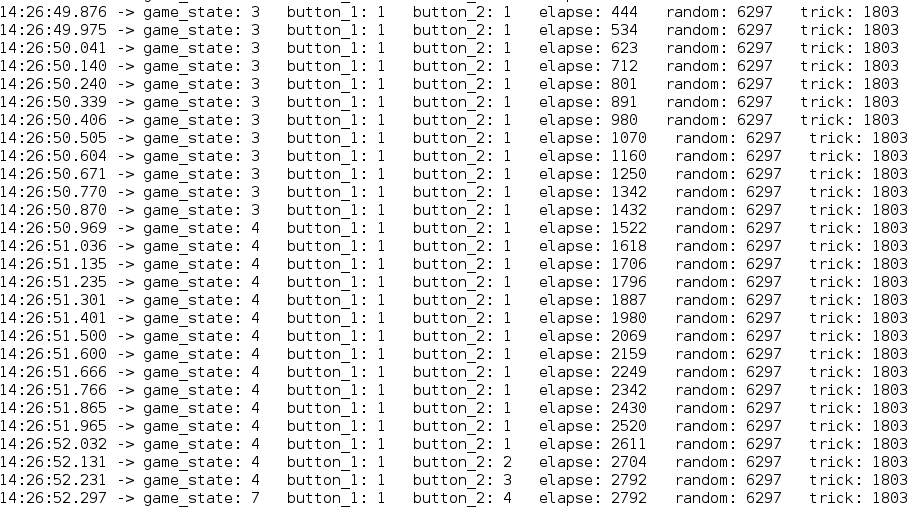
\includegraphics[scale=0.2]{03_serial}
      \caption{Typisk output frå serieporten mens spelet køyrer på arduinoen.}
    \end{center}
  \end{figure}

  Ein annan fordel med å bruke tilstandsmaskiner er at det var enkelt å utvide funksjonaliteten
  til programkomponentene. F.eks. dersom eg ønska ein ekstra meny eller ein ekstra spelmodus
  kunne eg legge til fleire tilstandar i spellogikkens tilstandsmaskin. Dersom eg ville
  utvida knappefunksjonaliteten til også å støtte ein ekstra tilstand du havner i
  dersom du trykker knappen ned lenge, så er dette triviellt å legge til. Du får mykje gratis,
  så dette er ein abstraksjon eg vil bruke meir av i framtida. \\


  Av problemer eg hadde kan eg nevne fleire ting som skyldast dårleg kunnskap om C++.
  Spesielt hadde eg problemer med \textit{scope}, og dette gjorde mitt første forsøk
  på å lage ein \textit{menucontroller}-klasse vanskeleg. Eg endte med å kun ha eitt lag av
  objekter, og ein flat struktur uten arv og hierarki på grunn av dette. \\

\end{document}
